\documentclass[tikz]{standalone}

\usepackage{icomma}

% tikz
\usepackage{tikz, pgfplots}
% i wish external worked but idk it sucks
%\usetikzlibrary{external}
%\tikzexternalize[prefix=figures/]

% for function graph
\usetikzlibrary{positioning}
\usetikzlibrary{shapes.geometric}
\usetikzlibrary{positioning}
\tikzset{
dot/.style = {circle, fill=#1, minimum size=5pt,
              inner sep=0pt, outer sep=0pt},
dot/.default = black % size of the circle diameter
}

 % for braces
\usetikzlibrary{decorations.pathreplacing}
% for hashing area
\usetikzlibrary{patterns}
% tableaux var, signe
% source https://www.sqlpac.com/fr/documents/latex-package-tkz-tab-tikz-tableaux-de-signes-et-de-variations-de-fonctions.html
\usepackage{tkz-tab}
%%%%%%%%%%%%%%%%%%%%%%%%%%%%%%
% SELF MADE COLORS
%%%%%%%%%%%%%%%%%%%%%%%%%%%%%%


\definecolor{myg}{RGB}{56, 140, 70}
\definecolor{myb}{RGB}{45, 111, 177}
\definecolor{myr}{RGB}{199, 68, 64}
\definecolor{mytheorembg}{HTML}{F2F2F9}
\definecolor{mytheoremfr}{HTML}{00007B}
\definecolor{mylenmabg}{HTML}{FFFAF8}
\definecolor{mylenmafr}{HTML}{983b0f}
\definecolor{mypropbg}{HTML}{f2fbfc}
\definecolor{mypropfr}{HTML}{191971}
\definecolor{myexamplebg}{HTML}{F2FBF8}
\definecolor{myexamplefr}{HTML}{88D6D1}
\definecolor{myexampleti}{HTML}{2A7F7F}
\definecolor{mydefinitbg}{HTML}{E5E5FF}
\definecolor{mydefinitfr}{HTML}{3F3FA3}
\definecolor{notesgreen}{RGB}{0,162,0}
\definecolor{myp}{RGB}{197, 92, 212}
\definecolor{mygr}{HTML}{2C3338}
\definecolor{myred}{RGB}{127,0,0}
\definecolor{myyellow}{RGB}{169,121,69}
\definecolor{myexercisebg}{HTML}{F2FBF8}
\definecolor{myexercisefg}{HTML}{88D6D1}
\definecolor{doc}{RGB}{0,60,110}

% manim colors because they're beautiful
% https://docs.manim.community/en/stable/reference/manim.utils.color.manim_colors.html

\definecolor{BLACK}{HTML}{000000}\definecolor{BLUE}{HTML}{58C4DD}\definecolor{BLUE_A}{HTML}{C7E9F1}\definecolor{BLUE_B}{HTML}{9CDCEB}\definecolor{BLUE_C}{HTML}{58C4DD}\definecolor{BLUE_D}{HTML}{29ABCA}\definecolor{BLUE_E}{HTML}{236B8E}\definecolor{DARKER_GRAY}{HTML}{222222}\definecolor{DARKER_GREY}{HTML}{222222}\definecolor{DARK_BLUE}{HTML}{236B8E}\definecolor{DARK_BROWN}{HTML}{8B4513}\definecolor{DARK_GRAY}{HTML}{444444}\definecolor{DARK_GREY}{HTML}{444444}\definecolor{GOLD}{HTML}{F0AC5F}\definecolor{GOLD_A}{HTML}{F7C797}\definecolor{GOLD_B}{HTML}{F9B775}\definecolor{GOLD_C}{HTML}{F0AC5F}\definecolor{GOLD_D}{HTML}{E1A158}\definecolor{GOLD_E}{HTML}{C78D46}\definecolor{GRAY}{HTML}{888888}\definecolor{GRAY_A}{HTML}{DDDDDD}\definecolor{GRAY_B}{HTML}{BBBBBB}\definecolor{GRAY_BROWN}{HTML}{736357}\definecolor{GRAY_C}{HTML}{888888}\definecolor{GRAY_D}{HTML}{444444}\definecolor{GRAY_E}{HTML}{222222}\definecolor{GREEN}{HTML}{83C167}\definecolor{GREEN_A}{HTML}{C9E2AE}\definecolor{GREEN_B}{HTML}{A6CF8C}\definecolor{GREEN_C}{HTML}{83C167}\definecolor{GREEN_D}{HTML}{77B05D}\definecolor{GREEN_E}{HTML}{699C52}\definecolor{GREY}{HTML}{888888}\definecolor{GREY_A}{HTML}{DDDDDD}\definecolor{GREY_B}{HTML}{BBBBBB}\definecolor{GREY_BROWN}{HTML}{736357}\definecolor{GREY_C}{HTML}{888888}\definecolor{GREY_D}{HTML}{444444}\definecolor{GREY_E}{HTML}{222222}\definecolor{LIGHTER_GRAY}{HTML}{DDDDDD}\definecolor{LIGHTER_GREY}{HTML}{DDDDDD}\definecolor{LIGHT_BROWN}{HTML}{CD853F}\definecolor{LIGHT_GRAY}{HTML}{BBBBBB}\definecolor{LIGHT_GREY}{HTML}{BBBBBB}\definecolor{LIGHT_PINK}{HTML}{DC75CD}\definecolor{LOGO_BLACK}{HTML}{343434}\definecolor{LOGO_BLUE}{HTML}{525893}\definecolor{LOGO_GREEN}{HTML}{87C2A5}\definecolor{LOGO_RED}{HTML}{E07A5F}\definecolor{LOGO_WHITE}{HTML}{ECE7E2}\definecolor{MAROON}{HTML}{C55F73}\definecolor{MAROON_A}{HTML}{ECABC1}\definecolor{MAROON_B}{HTML}{EC92AB}\definecolor{MAROON_C}{HTML}{C55F73}\definecolor{MAROON_D}{HTML}{A24D61}\definecolor{MAROON_E}{HTML}{94424F}\definecolor{ORANGE}{HTML}{FF862F}\definecolor{PINK}{HTML}{D147BD}\definecolor{PURE_BLUE}{HTML}{0000FF}\definecolor{PURE_GREEN}{HTML}{00FF00}\definecolor{PURE_RED}{HTML}{FF0000}\definecolor{PURPLE}{HTML}{9A72AC}\definecolor{PURPLE_A}{HTML}{CAA3E8}\definecolor{PURPLE_B}{HTML}{B189C6}\definecolor{PURPLE_C}{HTML}{9A72AC}\definecolor{PURPLE_D}{HTML}{715582}\definecolor{PURPLE_E}{HTML}{644172}\definecolor{RED}{HTML}{FC6255}\definecolor{RED_A}{HTML}{F7A1A3}\definecolor{RED_B}{HTML}{FF8080}\definecolor{RED_C}{HTML}{FC6255}\definecolor{RED_D}{HTML}{E65A4C}\definecolor{RED_E}{HTML}{CF5044}\definecolor{TEAL}{HTML}{5CD0B3}\definecolor{TEAL_A}{HTML}{ACEAD7}\definecolor{TEAL_B}{HTML}{76DDC0}\definecolor{TEAL_C}{HTML}{5CD0B3}\definecolor{TEAL_D}{HTML}{55C1A7}\definecolor{TEAL_E}{HTML}{49A88F}\definecolor{WHITE}{HTML}{FFFFFF}\definecolor{YELLOW}{HTML}{FFFF00}\definecolor{YELLOW_A}{HTML}{FFF1B6}\definecolor{YELLOW_B}{HTML}{FFEA94}\definecolor{YELLOW_C}{HTML}{FFFF00}\definecolor{YELLOW_D}{HTML}{F4D345}\definecolor{YELLOW_E}{HTML}{E8C11C}

% Schwartz
\renewcommand{\S}{\mathcal{S}} % \S est le signe paragraphe normalement

% corps
\newcommand{\C}{\mathcal{C}}
\newcommand{\R}{\mathbb{R}}
\newcommand{\Rnn}{\mathbb{R}^{2n}}
\newcommand{\Z}{\mathbb{Z}}
\newcommand{\N}{\mathbb{N}}
\newcommand{\Q}{\mathbb{Q}}

% domain
\newcommand{\D}{\mathcal{D}}

% order notations
\renewcommand{\O}{\mathcal{O}}

% japanese bracket
\newcommand{\japb}[1]{\langle #1 \rangle}

% arrows over partial derivatives
\newcommand{\lp}{\overleftarrow{\partial}}
\newcommand{\rp}{\overrightarrow{\partial}}

% quantization
\newcommand{\h}{\hbar}
\newcommand{\Opht}{\textrm{Op}_{\h}^{t}}
\newcommand{\Op}[2][\hbar]{\textrm{Op}_{#1}^{#2}}

% omega functions
\newcommand{\omegap}[2][\rho_0]{\omega(\partial_{#1},\partial_{#2})}
\newcommand{\omegar}[2][\rho_0]{\omega(#1,#2)}



\tikzset{
	every node/.style = {font=\Large}
}

\tikzset{
	every axis/.style = {clip=true, grid style = {opacity=.5}}
}

\begin{document}
%
	% page 1
	    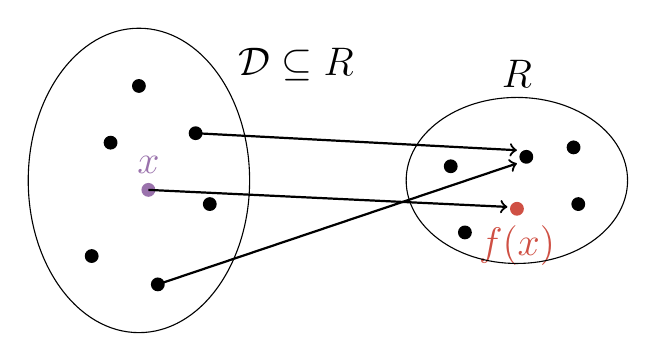
\begin{tikzpicture}[scale=1.2]
	        % domaine
	    	\coordinate (B) at (0,1);
	    	\coordinate (C) at (.1,.9);
	
	    	\node[dot=PURPLE, label=above:$\color{PURPLE}x$] at (C){};
	    	
	    	\node[ellipse, draw, label=above right:$\D \subseteq \R$, minimum height=110pt, minimum width=80pt] at (B){};
	
	        % codomaine
	    	\coordinate (D) at (4,.7);
	    	\node[dot=RED_E, label=below:$\color{RED_E}f(x)$] at (D){};
	    	\node[ellipse, draw, label=above:$\R$, minimum height=60pt, minimum width=80pt] at (4,1){};
	
		%maps
		
	    	\draw[thick, ->] (C) -- (3.9,.72);
	    	\draw[thick, ->] (.6,1.5) -- (4,1.32);
	    	\draw[thick, ->] (.2,-.1) -- (4,1.18);
	    	
	    	% morepoitns
	    	
	    	\node[dot=black] at (0, 2){};		    	
	    	\node[dot=black] at (.2,-.1){};
	    	\node[dot=black] at (.6,1.5){};
	    	\node[dot=black] at (.75,.75){};
	    	\node[dot=black] at (-.3,1.4){};
	    	\node[dot=black] at (-.5,.2){};
	    	%\node[dot=black] at (.1,.9){};
	    	
	    	
	    	\node[dot=black] at (4.65,.75){};
	    	\node[dot=black] at (4.1,1.25){};
	    	\node[dot=black] at (4.6,1.35){};
	    	\node[dot=black]  at (3.45,.45){};
	    	%\node[dot=black]  at (4,.7){};
	    	\node[dot=black]  at (3.3,1.15){};
	
	    \end{tikzpicture}
	    
	    % page 2
		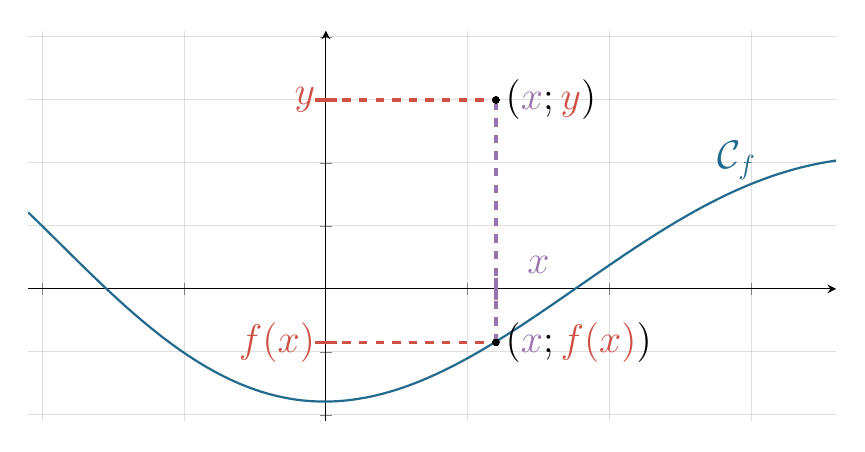
\begin{tikzpicture}[>=stealth]
			\begin{axis}[xmin = -2.1, xmax=3.6, xtick={-2, ..., 5},xticklabel=\empty, ymin=-2.1, ymax=4.1, ytick={-2, ...,4}, yticklabel=\empty, axis x line=middle, axis y line=middle, axis line style=->, grid=both, x = 1.8cm, y=.8cm]
				\addplot[no marks, BLUE_E, thick, -] expression[domain=-2.1: 4.1, samples=100]{(x+3.5)*(x+2.5)*(x-3.5)*(x-4.5)*(x-5.5)/200 + 2}
				node[pos=.86, above]{$\mathcal{C}_f $};
				
				\addplot[black, mark=*, mark size = 1] (1.2,3) node[above, right] {$({\color{PURPLE}x};{\color{RED_E}y})$};
				\addplot[black, mark=*, mark size = 1] (1.2,-.85) node[below, right] {$\bigl({\color{PURPLE}x};{\color{RED_E}f(x)}\bigr)$};
				
				\draw[PURPLE, dashed, very thick] (axis cs:1.2, -.85) -- (axis cs:1.2,3);
				\addplot[RED_E, dashed, very thick, domain = 0:1.2, samples=2] {3};
				\addplot[RED_E, dashed, very thick, domain = 0:1.2, samples=2] {-.85};
				
				\addplot[PURPLE, very thick, mark=|, mark size = 4] (1.2,0); % x cross
				\addplot[PURPLE] (1.5,0) node[above=2pt] {$x$}; % x label
				\addplot[RED_E, very thick, mark=-, mark size = 4] (0,3) node[left] {$y$};
				\addplot[RED_E, very thick, mark=-, mark size = 4] (0,-.85) node[left] {$f(x)$};
			\end{axis}
		
		\end{tikzpicture}
		
		%page 3
		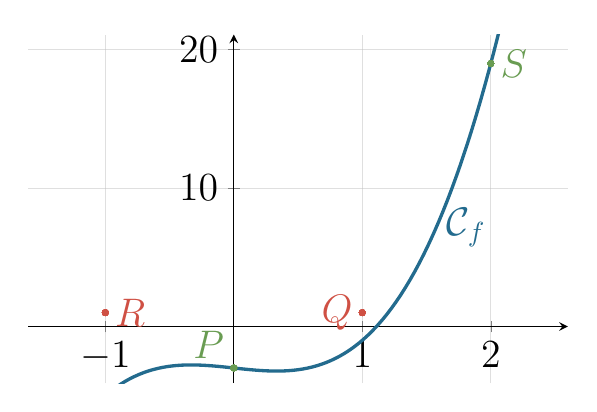
\begin{tikzpicture}[>=stealth]
			\begin{axis}[xmin = -1.6, xmax=2.6, ymin=-4.1, ymax=21.1, axis x line=middle, axis y line=middle, axis line style=->, grid=both,y = 5pt
			]
				\addplot[no marks, BLUE_E, very thick, -] expression[domain=-1.1: 2.5, samples=100]{3*x^3 -x -3}
				node[pos=.3, right]{$\mathcal{C}_f$};
				
				\addplot[GREEN_E, mark=*, mark size = 1] (0,-3) node[above left] {$P$};
				\addplot[RED_E, mark=*, mark size = 1] (1,1) node[below, left] {$Q$};
				\addplot[RED_E, mark=*, mark size = 1] (-1,1) node[below, right] {$R$};
				\addplot[GREEN_E, mark=*, mark size = 1] (2,19) node[below, right] {$S$};
			\end{axis}
		
		\end{tikzpicture}
		
		% page 4
		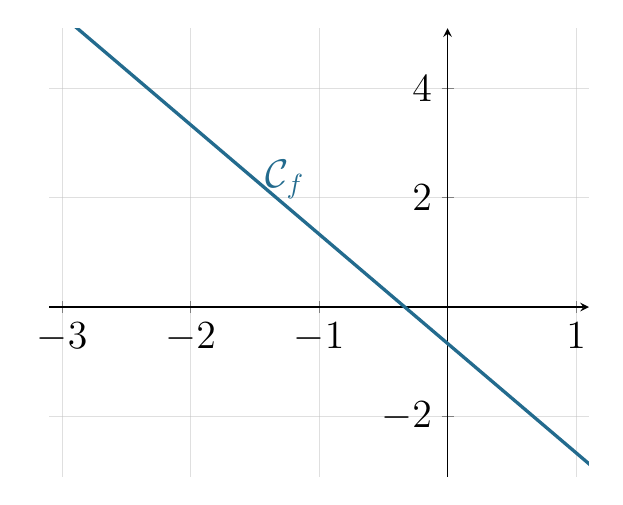
\begin{tikzpicture}[>=stealth]
			\begin{axis}[xmin = -3.1, xmax=1.1, ymin=-3.1, ymax=5.1, axis x line=middle, axis y line=middle, axis line style=->, grid=both,
			grid style = {opacity=.5},
			]
				\addplot[no marks, BLUE_E, very thick, -] expression[domain=-3:2, samples=2]{-2/3 - 2*x}
				node[pos=.3, right]{$\mathcal{C}_f$};
			\end{axis}
		
		\end{tikzpicture}
		
		% page 5
		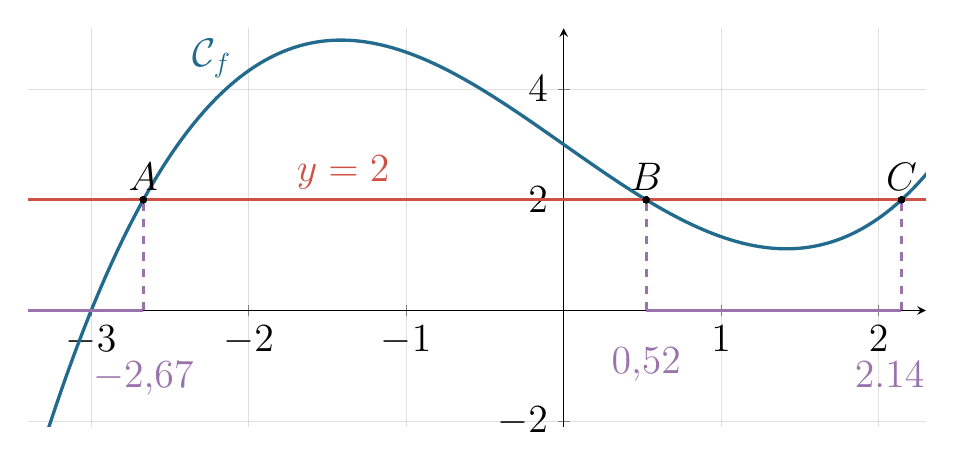
\begin{tikzpicture}[>=stealth]
			\begin{axis}[xmin = -3.4, xmax=2.3, ymin=-2.1, ymax=5.1, axis x line=middle, axis y line=middle, axis line style=->, grid=both,
			grid style = {opacity=.5},
			x=2cm,
			xtick={-3, -2, ..., 2},
			y=20pt,
			]
				\addplot[no marks, BLUE_E, very thick, -] expression[domain=-4:3, samples=200]{x^3 /3 - 2*x +3}
				node[pos=.55, above=5pt]{$\mathcal{C}_f$};
				
				\addplot[no marks, RED_E, very thick, -] expression[domain=-5:3, samples=2]{2}
				node[pos=.45, above]{$y=2$};
				
				
				\addplot[black, mark=*, mark size = 1] (-2.6691, 2) node[above] {$A$};
				\addplot[black, mark=*, mark size = 1] (0.52398, 2) node[above] {$B$};
				\addplot[black, mark=*, mark size = 1] (2.1451, 2) node[above] {$C$};
				
				\draw[PURPLE, dashed, very thick] (axis cs:-2.6691, 0) -- (axis cs:-2.6691, 2);
				\draw[PURPLE, dashed, very thick] (axis cs:0.52398, 0) -- (axis cs:0.52398, 2);
				\draw[PURPLE, dashed, very thick] (axis cs:2.1451, 0) -- (axis cs:2.1451, 2);
				
				\addplot[PURPLE] (-2.6691,0) node[below=15pt] {$-2,67$};					
				\addplot[PURPLE] (0.52398,0) node[below=10pt] {$0,52$};					
				\addplot[PURPLE] (2.07,0) node[below=15pt] {$2.14$};
				
				
				\addplot[no marks, PURPLE, very thick, -] expression[domain=-3.4:-2.67, samples=2]{0};
				\addplot[no marks, PURPLE, very thick, -] expression[domain=.52:2.14, samples=2]{0};
			\end{axis}
		\end{tikzpicture}
		
		% page 6
		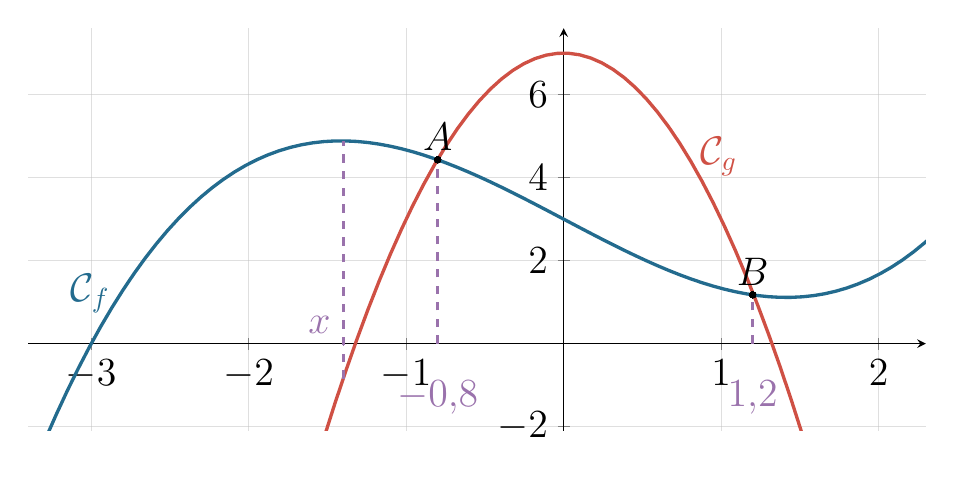
\begin{tikzpicture}[>=stealth]
			\begin{axis}[xmin = -3.4, xmax=2.3, ymin=-2.1, ymax=7.6, axis x line=middle, axis y line=middle, axis line style=->, grid=both,
			grid style = {opacity=.5},
			x=2cm,
			xtick={-3, -2, ..., 2},
			y=15pt,
			]
				\addplot[no marks, BLUE_E, very thick, -] expression[domain=-4:3, samples=100]{x^3 /3 - 2*x +3}
				node[pos=.4, above=8pt]{$\mathcal{C}_f$};
				\addplot[no marks, RED_E, very thick, -] expression[domain=-4:3, samples=100]{-4*x^2 + 7}
				node[pos=.68, above=10pt]{$\mathcal{C}_g$};
			
				\addplot[black, mark=*, mark size = 1] (-.8, 4.43) node[above] {$A$};
				\addplot[black, mark=*, mark size = 1] (1.2, 1.176) node[above] {$B$};
				
				\draw[PURPLE, dashed, very thick] (axis cs:-.8, 0) -- (axis cs:-.8, 4.43);
				\draw[PURPLE, dashed, very thick] (axis cs:1.2, 0) -- (axis cs:1.2, 1.176);
				
				\addplot[PURPLE] (-.8,0) node[below=10pt] {$-0,8$};					
				\addplot[PURPLE] (1.2,0) node[below=10pt] {$1,2$};
				
				
				\addplot[PURPLE, mark=|, mark size = 1] (-1.4, 0);
				\addplot[PURPLE] (-1.55, 0) node[above] {$x$};
				\draw[PURPLE, dashed, very thick] (axis cs:-1.4, -.84) -- (axis cs:-1.4, 4.8853);
			\end{axis}
		\end{tikzpicture}
		
		% page 7
		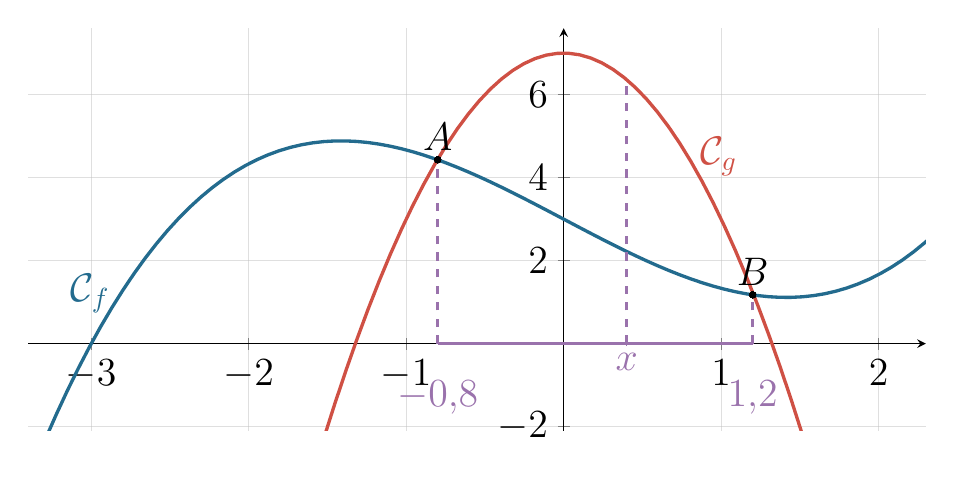
\begin{tikzpicture}[>=stealth]
			\begin{axis}[xmin = -3.4, xmax=2.3, ymin=-2.1, ymax=7.6, axis x line=middle, axis y line=middle, axis line style=->, grid=both,
			grid style = {opacity=.5},
			x=2cm,
			xtick={-3, -2, ..., 2},
			y=15pt,
			]
			\addplot[no marks, BLUE_E, -, very thick] expression[domain=-4:3, samples=100]{x^3 /3 - 2*x +3}
			node[pos=.4, above=8pt]{$\mathcal{C}_f$};
			\addplot[no marks, RED_E, -,  very thick] expression[domain=-4:3, samples=100]{-4*x^2 + 7}
			node[pos=.68, above=10pt]{$\mathcal{C}_g$};
		
			\addplot[black, mark=*, mark size = 1] (-.8, 4.43) node[above] {$A$};
			\addplot[black, mark=*, mark size = 1] (1.2, 1.176) node[above] {$B$};
			
			\draw[PURPLE, dashed, very thick] (axis cs:-.8, 0) -- (axis cs:-.8, 4.43);
			\draw[PURPLE, dashed, very thick] (axis cs:1.2, 0) -- (axis cs:1.2, 1.176);
			
			\addplot[PURPLE] (-.8,0) node[below=10pt] {$-0,8$};					
			\addplot[PURPLE] (1.2,0) node[below=10pt] {$1,2$};
			
			
			\addplot[PURPLE, mark=|, mark size = 1] (.4, 0) node[below] {$x$};
			\draw[PURPLE, dashed, very thick] (axis cs:.4, 0) -- (axis cs:.4, 6.36);
			
			
			\addplot[no marks, PURPLE, very thick, -] expression[domain=-.8:1.2, samples=2]{0};
		\end{axis}
	\end{tikzpicture}
	
	% page 8
		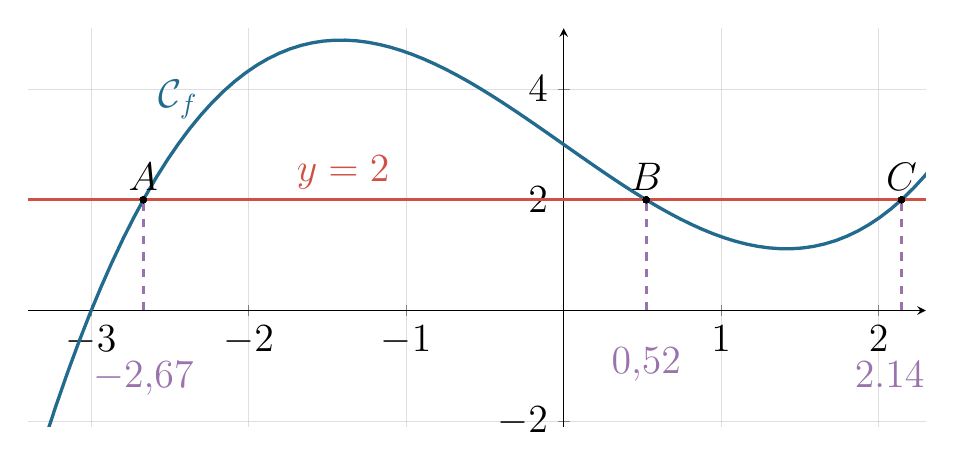
\begin{tikzpicture}[>=stealth]
			\begin{axis}[xmin = -3.4, xmax=2.3, ymin=-2.1, ymax=5.1, axis x line=middle, axis y line=middle, axis line style=->, grid=both,
			grid style = {opacity=.5},
			x=2cm,
			xtick={-3, -2, ..., 2},
			y=20pt,
			]
				\addplot[no marks, BLUE_E, very thick, -] expression[domain=-4:3, samples=100]{x^3 /3 - 2*x +3}
				node[pos=.52, above=5pt]{$\mathcal{C}_f$};
				
				\addplot[no marks, RED_E, very thick, -] expression[domain=-5:3, samples=2]{2}
				node[pos=.45, above]{$y=2$};
				
				
				\addplot[black, mark=*, mark size = 1] (-2.6691, 2) node[above] {$A$};
				\addplot[black, mark=*, mark size = 1] (0.52398, 2) node[above] {$B$};
				\addplot[black, mark=*, mark size = 1] (2.1451, 2) node[above] {$C$};
				
				\draw[PURPLE, dashed, very thick] (axis cs:-2.6691, 0) -- (axis cs:-2.6691, 2);
				\draw[PURPLE, dashed, very thick] (axis cs:0.52398, 0) -- (axis cs:0.52398, 2);
				\draw[PURPLE, dashed, very thick] (axis cs:2.1451, 0) -- (axis cs:2.1451, 2);
				
				\addplot[PURPLE] (-2.6691,0) node[below=15pt] {$-2,67$};					
				\addplot[PURPLE] (0.52398,0) node[below=10pt] {$0,52$};					
				\addplot[PURPLE] (2.07,0) node[below=15pt] {$2.14$};
			\end{axis}
		\end{tikzpicture}
		
		% page 9
		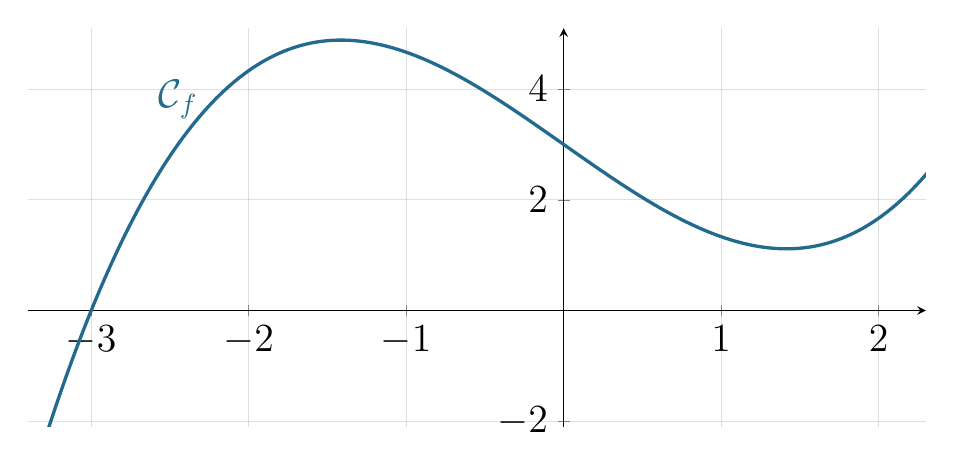
\begin{tikzpicture}[>=stealth]
			\begin{axis}[xmin = -3.4, xmax=2.3, ymin=-2.1, ymax=5.1, axis x line=middle, axis y line=middle, axis line style=->, grid=both,
			grid style = {opacity=.5},
			x=2cm,
			xtick={-3, -2, ..., 2},
			y=20pt,
			]
				\addplot[no marks, BLUE_E, very thick, -] expression[domain=-4:3, samples=200]{x^3 /3 - 2*x +3}node[pos=.52, above=5pt]{$\C_f$};
			\end{axis}
		\end{tikzpicture}
		%page 10
	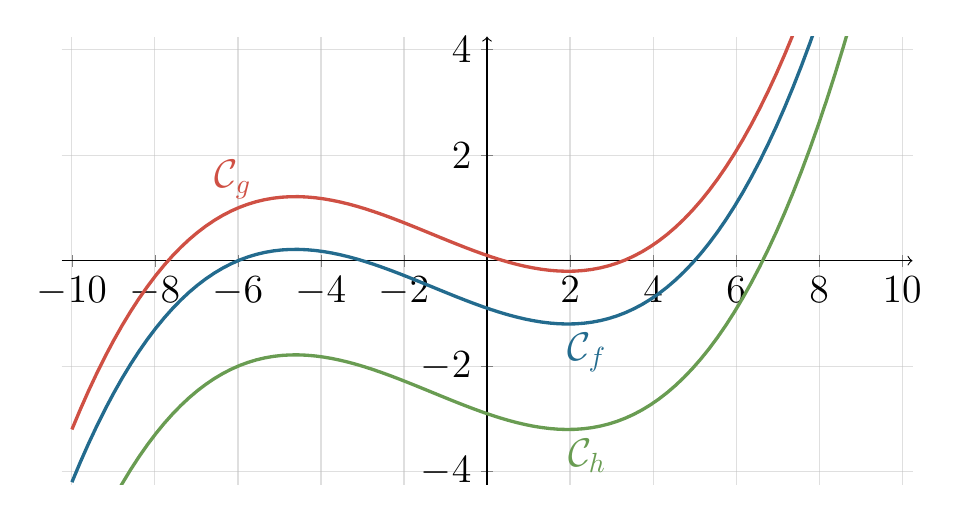
\begin{tikzpicture}[scale=1]
		\begin{axis}[xmin = -10.25, xmax=10.25, ymin=-4.25, ymax=4.25, axis x line=middle, axis y line=middle, axis line style=->, grid=both,
		grid style = {opacity=.5},
	    	x=15pt,
	    	]
		% g cos
		\addplot[no marks, BLUE_E, -, very thick] expression[domain=-10:10, samples=100]{.01*(x+6)*(x+3)*(x-5)}
		node[pos=.5, below]{$\mathcal{C}_f$};
		\addplot[no marks, RED_E, -, very thick] expression[domain=-10:10, samples=100]{.01*(x+6)*(x+3)*(x-5)+1}
		node[pos=.2, above]{$\mathcal{C}_g$};
		\addplot[no marks, GREEN_E, -, very thick] expression[domain=-10:10, samples=100]{.01*(x+6)*(x+3)*(x-5)-2}
		node[pos=.5,below]{$\mathcal{C}_h$};
		\end{axis}
	\end{tikzpicture}
	%page 11
	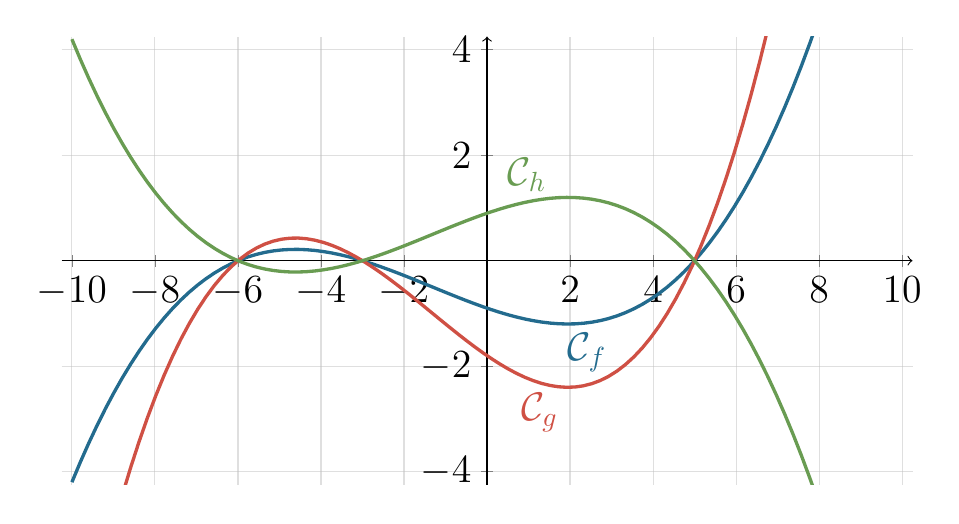
\begin{tikzpicture}[scale=1]
		\begin{axis}[xmin = -10.25, xmax=10.25, ymin=-4.25, ymax=4.25, axis x line=middle, axis y line=middle, axis line style=->, grid=both,,
		grid style = {opacity=.5},
	    	x=15pt,
	    	]
		% g cos
		\addplot[no marks, BLUE_E, -, very thick] expression[domain=-10:10, samples=100]{.01*(x+6)*(x+3)*(x-5)}
		node[pos=.5, below]{$\mathcal{C}_f$};
		\addplot[no marks, RED_E, -, very thick] expression[domain=-10:10, samples=100]{.02*(x+6)*(x+3)*(x-5)}
		node[pos=.4, below]{$\mathcal{C}_g$};
		\addplot[no marks, GREEN_E, -, very thick] expression[domain=-10:10, samples=100]{-.01*(x+6)*(x+3)*(x-5)}
		node[pos=.45, above]{$\mathcal{C}_h$};
		\end{axis}
	\end{tikzpicture}
	
	% page 12
	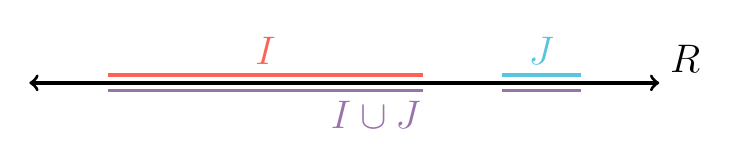
\begin{tikzpicture}
		\draw[very thick, black, <->] (-4, 0) -- (4, 0) node[above right] {$\R$};
		
		\draw[very thick, RED, -] (-3, .1) -- (1, .1) node[pos=.5, above] {$I$};
		\draw[very thick, BLUE, -] (2, .1) -- (3, .1) node[pos=.5, above] {$J$};
		
		\draw[very thick, PURPLE, -] (2, -.1) -- (3, -.1);
		\draw[very thick, PURPLE, -] (-3, -.1) -- (1, -.1) node[pos=.85, below] {$I\cup J$};
	\end{tikzpicture}
%
\end{document}